\documentclass[a4paper,10pt]{article}
\usepackage{fancyhdr}
\usepackage[spanish,activeacute]{babel}
%usepackage{algorithm}
%\usepackage{algpseudocode}
\pagestyle{fancy}
\frenchspacing
\usepackage[dvips]{graphicx}
\usepackage[dvips]{geometry}
\usepackage[usenames]{color}
\usepackage{colortbl}
\usepackage{amssymb}
\usepackage{caratula}
\usepackage{hyperref}
\usepackage[utf8]{inputenc}
\usepackage{array}
\usepackage{float}

%Colores
\definecolor{tcA}{gray}{0.90}

%Traducción de instrucciones
%\algrenewcommand\algorithmicwhile{\textbf{mientras}}
%\algrenewcommand\algorithmicdo{\textbf{hacer}}
%\algrenewcommand\algorithmicend{\textbf{fin}}
%\algrenewcommand\algorithmicprocedure{\textbf{Procedimiento}}
%\algrenewcommand\algorithmicfor{\textbf{para}}
%\algrenewcommand\algorithmicif{\textbf{si}}
%\algrenewcommand\algorithmicelse{\textbf{sino}}
%\algrenewcommand\algorithmicthen{\textbf{entonces}}
%\algrenewcommand\algorithmicfunction{\textbf{Funci\'on}}
%\algnewcommand\algorithmicto{\textbf{hasta}}

\lhead{\textbf{Teoría de las comunicaciones - TP1}}
\rhead{Capello - Hernandez - Laurito}
\lfoot{Taller de Wiretapping}
\rfoot{\thepage}
\cfoot{ }
\renewcommand{\headrulewidth}{0.6pt}
\renewcommand{\footrulewidth}{0.4pt}
\addtolength{\textwidth}{2cm}
\addtolength{\hoffset}{-0.8cm}
\fancyheadoffset{1cm}
\fancyfootoffset{1cm}

\begin{document}

\materia{Teor'ia de las Comunicaciones}
\submateria{Primer Cuatrimestre de 2013}
\titulo{Taller de Wiretapping}
%\subtitulo{}
\grupo{Grupo:}
\integrante{Mat\'ias Capello}{006/02}{matiascapello@gmail.com}
\integrante{Santiago Hern'andez}{48/11}{santi-hernandez@hotmail.com}
\integrante{Andr'es Laurito}{27/11}{andy.laurito@hotmail.com}

\begin{titlepage}
\maketitle
\thispagestyle{empty}
\end{titlepage} 

\pagebreak
\tableofcontents

\pagebreak
\listoffigures

\pagebreak
\thispagestyle{fancy}

\section*{\centering Abstract}
{\em
Las redes inform'aticas pueden tener una complejidad tal que describir la disposici'on, participaci'on y rol de los nodos de una red sin saber nada de ella pueda ser una tarea dificil.	\\
\indent	El objetivo de este trabajo es lograr determinar cuales son nodos distinguidos en una red y un panorama de la topolog'ia y din'amica de la misma de una manera sencilla.	\\
\indent	En este experimento se captur'o y analiz'o el tr'afico de paquetes ARP enviados en una red empresarial en pos de lograr el objetivo. Los an'alisis realizados estan basados en histogramas de direcciones IP destino y fuente, diagramas de actividad a lo largo del tiempo, el c'alculo de la entrop'ia de la red y la informaci'on de las direcciones, y el gráfico de la red como un digrafo. Para esto se estudi'o y prob'o el protocolo ARP previamente.	\\
\indent	Se encontr'o que si bien la mayor'ia de la red presenta un comportamiento de acuerdo al esperado de acuerdo a la teor'ia, aparecieron nodos cuyo comportamiento no solo es distinguido, si no que no se condiciona a lo esperado.	\\
\indent	A partir de los resultados concluimos que el an'alisis de la red realizado en base a los mensajes ARP sirve para hallar nodos distinguidos en la red y obtener un panorama de la topolog'ia de la misma, no es suficiente para comprender la red y su din'amica en su totatiladad ya que se presentan fen'omenos y nodos distinguidos cuya participaci'on y rol no logramos determinar.
}
%~ {\em
%~ En el presente trabajo se analizar'a el protocolo ARP. En la primera parte se muestra la implementaci'on de un cliente ARP, utilizando Scapy. Se realizan varias pruebas utilizando diferentes direcciones para ver que respuesta se obtiene. Para la segunda parte, se implementa una funci'on para escuchar pasivamente una red por un lapso de dos horas, capturando los mensajes ARP. En base a los datos recojidos, se definen dos modelos para el c'alculo de la entrop'ia de la red y se realizan gr'aficos que permiten analizarla: topol'ogico, histogramas y actividad en el tiempo. El primer modelo tiene como conjunto de s'imbolos las direcciones IP destino que aparecieron en los paquetes ARP capturados. En el segundo modelo, los s'imbolos son las direcciones de IP origen. Como resultado, se logr'o detectar varios nodos particulares: El router, algunos que s'olo realizan solicitudes con su propia IP en forma cont'inua, y otros con alta actividad.
%~ %end italics mode
%~ }
\vspace*{5 mm}

Palabras clave: red, ARP, nodos distinguidos, topolog'ia.


\section{Introducci'on}
\label{intro1:}

El objetivo de este trabajo pr'actico es abordar algunas nociones de nivel de enlace, poniendo fundamentalmente el foco en el v'inculo con la capa superior y desarrollando un acercamiento anal'itico. El objetivo ser'a analizar de manera interactiva el protocolo \textbf{ARP} y sacar algunas conclusiones de c'omo se comportan los hosts en un segumento de red determinado.

\subsection{ARP - Address Resolution Protocol}

El protocolo \textbf{ARP} tiene un papel clave entre los protocolos de capa de Internet relacionados con el protocolo TCP/IP, ya que permite que se conozca la direcci'on f'isica de una tarjeta de interfaz de red correspondiente a una direcci'on IP. Por eso se llama Protocolo de Resoluci'on de Direcci'on (en ingl'es \textbf{ARP} significa Address Resolution Protocol).

\vspace*{5 mm}
Cada equipo conectado a la red tiene un n'umero de identificaci'on de 48 bits. 'Este es un n'umero 'unico establecido en la f'abrica en el momento de fabricaci'on de la tarjeta. Sin embargo, la comunicaci'on en Internet no utiliza directamente este n'umero (ya que las direcciones de los equipos deber'ian cambiarse cada vez que se cambia la tarjeta de interfaz de red), sino que utiliza una direcci'on l'ogica asignada por un organismo: la direcci'on IP.

\vspace*{5 mm}
Para que las direcciones f'isicas se puedan conectar con las direcciones l'ogicas, el protocolo \textbf{ARP} interroga a los equipos de la red para averiguar sus direcciones f'isicas y luego crea una tabla de b'usqueda entre las direcciones l'ogicas y f'isicas en una memoria cach'e.

\vspace*{5 mm}
Cuando un equipo debe comunicarse con otro, consulta la tabla de b'usqueda. Si la direcci'on requerida no se encuentra en la tabla, el protocolo \textbf{ARP} env'ia una solicitud a la red. Todos los equipos en la red comparan esta direcci'on l'ogica con la suya. Si alguno de ellos se identifica con esta direcci'on, el equipo responder'a al \textbf{ARP}, que almacenar'a el par de direcciones en la tabla de b'usqueda, y, a continuaci'on, podr'a establecerse la comunicaci'on. 

\vspace*{5 mm}
La Figura 1 muestra el formato del paquete \textbf{ARP} para el mapero de direcci'on IP-a-Ethernet. De hecho, \textbf{ARP} puede ser utilizado para muchos otros tipos de mapeos las mayores diferencias se dan en los tama\~nos de direcci'on. Adem'as de los OP y las direcciones de capa de enlace de ambos origen y destino, el paquete contiene:

\begin{itemize}
	\item Un campo HardwareType, que especifica el tipo de red f'isica (por ejemplo, Ethernet).
	\item Un campo ProtocolType, que especifica el protocolo de la capa superior (por ejemplo, IP).
	\item Campos HLen (hardware address length) y PLen (protocol address length), que especifican las longitudes de la direcci'on de capa de enlace y la direcci'on de la capa superior, respectivamente.
	\item Un campo Operation, que especifica si se trata de una solicitud o una respuesta.
	\item Las direcciones de origen y destino del hardware (Ethernet) y protocolo (IP).
\end{itemize}

\begin{figure}[!hbp]
\begin{center}
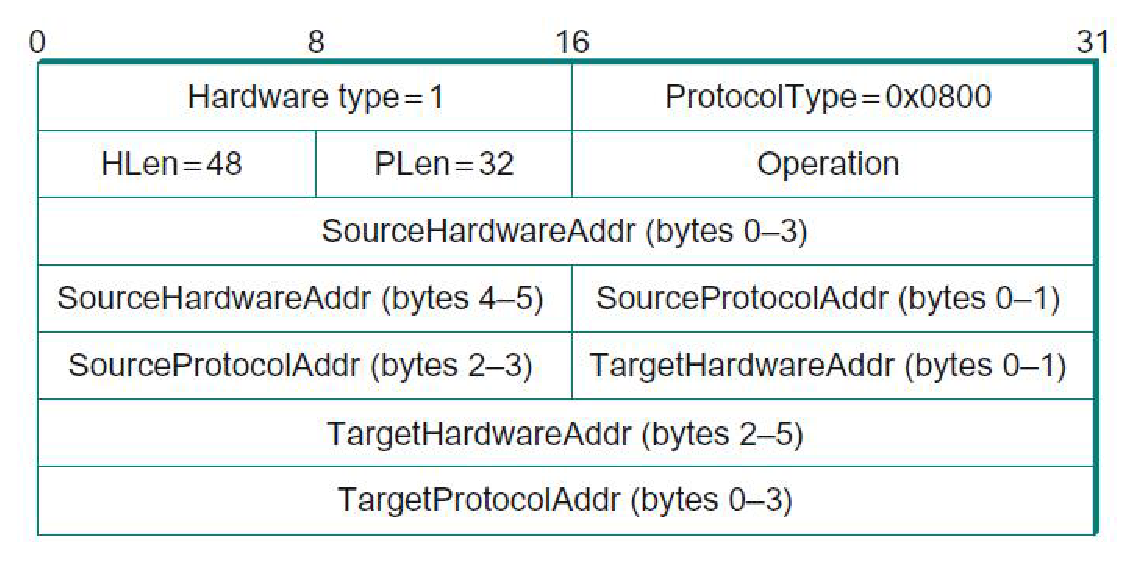
\includegraphics[width=12cm]{figura1.eps}
\end{center}
\caption{Figura 1 - Formato del paquete ARP para el mapeo de direcciones IP a direcciones Ethernet} \label{figura1}
\end{figure}

\subsection{Entrop'ia - Informaci'on}

En el 'ambito de la teor'ia de la informaci'on la entrop'ia, tambi'en llamada entrop'ia de la informaci'on y entrop'ia de Shannon (en honor a Claude E. Shannon), mide la incertidumbre de una fuente de informaci'on.

\vspace*{5 mm}
La entrop'ia tambi'en se puede considerar como la cantidad de informaci'on promedio que contienen los s'imbolos usados. Los s'imbolos con menor probabilidad son los que aportan mayor informaci'on; por ejemplo, si se considera como sistema de s'imbolos a las palabras en un texto, palabras frecuentes como \texttt{que}, \texttt{el}, \texttt{a} aportan poca informaci'on, mientras que palabras menos frecuentes como \texttt{corren}, \texttt{ni\~no}, \texttt{perro} aportan m'as informaci'on. Si de un texto dado borramos un \texttt{que}, seguramente no afectar'a a la comprensi'on y se sobreentender'a, no siendo as'i si borramos la palabra \texttt{ni\~no} del mismo texto original. Cuando todos los s'imbolos son igualmente probables (distribuci'on de probabilidad plana), todos aportan informaci'on relevante y la entrop'ia es m'axima.

\vspace*{5 mm}
El concepto de entrop'ia es usado en termodin'amica, mec'anica estad'istica y teor'ia de la informaci'on. En todos los casos la entrop'ia se concibe como una \textit{medida del desorden} o la \textit{peculiaridad de ciertas combinaciones}. La entrop'ia puede ser considerada como una medida de la incertidumbre y de la informaci'on necesarias para, en cualquier proceso, poder acotar, reducir o eliminar la incertidumbre. Resulta que el concepto de informaci'on y el de entrop'ia est'an ampliamente relacionados entre s'i, aunque se necesitaron a\~nos de desarrollo de la mec'anica estad'istica y de la teor'ia de la informaci'on antes de que esto fuera percibido.

\vspace*{5 mm}
Shannon ofrece una definici'on de entrop'ia que satisface las siguientes afirmaciones:

\begin{itemize}
	\item La medida de informaci'on debe ser proporcional (continua). Es decir, el cambio peque\~no en una de las probabilidades de aparici'on de uno de los elementos de la se\~nal debe cambiar poco la entrop'ia.
	\item Si todos los elementos de la se\~nal son equiprobables a la hora de aparecer, entonces la entrop'ia ser'a m'axima.	
\end{itemize}

\subsubsection{Definici'on Formal}

Supongamos que un fen'omeno (variable aleatoria) tiene un grado de indeterminaci'on inicial igual a k (k estados posibles) y supongamos todos los estados equiprobables, entonces la probabilidad p de que se d'e una de esas combinaciones ser'a 1/k. Podemos representar entonces la expresi'on  $c_{i}$ como:

\vspace*{5 mm}
$c_{i} = log_{2}(k) = log_{2}\left[ 1 \div (1 \div k)\right] = -log_{2}(p)$
\\

Si ahora cada uno de los k estados tiene una probabilidad $p_{i}$, entonces la entrop'ia vendr'a dada por la suma ponderada de la cantidad de informaci'on:

\vspace*{5 mm}
$H = -p_{1}log_{2}(p_{1}) - p_{2}log_{2}(p_{2}) - ... -p_{k}log_{2}(p_{k}) = -\sum^{k}_{i=1} p_{i}log_{2}(p_{i})$
\\

Por lo tanto, la entrop'ia de un mensaje X, denotado por H(X), es el valor medio ponderado de la cantidad de informaci'on de los diversos estados del mensaje:

\vspace*{5 mm}
$H(X) = -\sum_{i} p(x_{i})log_{2}p(x_{i})$
\\

\section{Desarrollo}
\label{desarrollo1:}
\subsection{Primera consigna: Implementaci'on de un cliente ARP}
\label{expli1:}

Se utiliz'o \textit{Scapy} para implementar un script que reciba una direcci'on IP, realice un pedido de su MAC Address y lo devuelva.

La funci'on implementada para resolver esto es \texttt{preguntarMAC}, que recibe una direcci'on IP por par'ametro

Dentro de dicha funci'on se ejecuta lo siguiente:

\vspace*{5 mm}
\texttt{mensajeARP = srp1(Ether(dst="ff:ff:ff:ff:ff:ff")/ARP(pdst=ip),timeout=2)}
\vspace*{5 mm}

Mediante srp1, se env'ia el paquete ARP en broadcast y se acepta solo la primer respuesta (suponemos que solo uno contesta ya que solo uno debería tener la ip). \texttt{Ether(dst="ff:ff:ff:ff:ff:ff")} es para mandarlo en modo broadcast y \texttt{ARP(pdst=ip)}, la IP de la que le pregunto su MAC Address.

\vspace*{5 mm}
Se prob'o esta funcionalidad con diferentes direcciones de IP, para analizar el resultado obtenido:

\begin{itemize}
	\item Direcci'on ip existente: Se obtiene la respuesta con la dirección MAC.
	\item Direcci'on ip inexistente: No hay respuesta, se cae por timeout.
	\item Direcci'on ip de la m'aquina origen: No hay respuesta, se cae por timeout.
	\item Direcci'on ip Broadcast: No hay respuesta, se cae por timeout.
\end{itemize}

Tambi'en se probaron los siguientes casos con scapy obteniendo estos resultados:

\begin{itemize}
	\item Direcci'on ip existente con su MAC address: Se obtiene la respuesta con la dirección MAC.
	\item Direcci'on ip existente con la MAC address "00:00:00:00:00:00": No hay respuesta, se cae por timeout.
	\item Direcci'on ip existente con una MAC address distinta a la suya y a la de broadcast: No hay respuesta, se cae por timeout.
	\item Direcci'on ip de nuestro router con nuestra MAC address y una IP distinta a la nuestra como source: Se obtiene la respuesta con la dirección MAC normalmente. No notamos cambios.
	\item Direcci'on ip equivocada a una MAC address conocida: No hay respuesta, se cae por timeout.
\end{itemize}

\subsection{Segunda consigna: Capturando tr'afico}
\label{expli1:}

Para la primera parte se nos ped'ia realizar un programa que escuche en la red por un per'iodo de tiempo y capture los mensajes ARP que circulen por la misma.

\vspace*{5 mm}

Para ello utilizamos la funci'on de Scapy \texttt{sniff} de la siguiente manera:

\vspace*{5 mm}

\texttt{sniff(prn=arp\_monitor\_callback, filter=''arp'', store=0)}

\vspace*{5 mm}

El par'ametro \texttt{store} se setea en 0 para que la funci'on \texttt{sniff()} no guarde nada (como lo har'ia de otra manera) y por lo tanto corra de forma ilimitada. El par'ametro \texttt{filter} se usa para mejorar la performance cuando hay alta carga de datos: El filtro se aplica dentro del kernel, por lo que Scapy s'olo ver'a trafico ARP.

\vspace*{5 mm}

La funci'on callback \texttt{arp\_monitor\_callback} se aplica a los paquetes que se sniffean, y se define asi:

\vspace*{5 mm}

\texttt{def arp\_monitor\_callback(pkt):}

\hspace*{3 mm}	\texttt{global salida}
	
\hspace*{3 mm}	\texttt{if ARP in pkt and pkt[ARP].op in (1,2):}
		
\hspace*{6 mm}			\texttt{salida.write(pkt.sprintf(''\%ARP.hwsrc\% \%ARP.psrc\% \%ARP.hwdst\% \%ARP}
			
\hspace*{6 mm}			\texttt{.pdst\% '')+str(datetime.now())+'$\setminus$ n')}
			
\hspace*{6 mm}			\texttt{return pkt.sprintf(''\%ARP.hwsrc\% \%ARP.psrc\% \%ARP.hwdst\% \%ARP.pdst\%'')}

\vspace*{5 mm}

La idea es que si los paquetes ARP son de tipo \texttt{who-has} o \texttt{is-at}, guarda en el archivo de salida y muestra por pantalla los datos de MAC source, IP source, MAC dest e IP dest. Datos que podr'an usarse luego para obtener informaci'on de la red.

\vspace*{5 mm}

Para la segunda parte de esta consigna se pide analizar la entrop'ia de la red. Para esto primero se dej'o corriendo el script anterior para capturar una buena cantidad de paquetes ARP en una red con tr'afico considerable. El lapso de tiempo usado para la captura fue de 2 horas. 

\vspace*{5 mm}

Se plantearon dos diferentes modelos para la fuente de informaci'on: En el primero, se defini'o como conjunto de s'imbolos a las direcciones de IP destino que aparecieran en los paquetes ARP capturados. La idea ser'ia la de poder distinguir direcciones muy solicitadas de otras poco buscadas. El segundo modelo una como s'imbolos a las direcciones de IP origen. Esta vez la idea es caracterizar a los nodos por generar gran cantidad o poca cantidad de requests ARP.

\vspace*{5 mm}

Para cada modelo el calculo consiste en obtener la probabilidad estad'istica de cada simbolo sobre el total y en base a eso obtener la informaci'on de cada s'imbolo y la entrop'ia de la fuente con las f'ormulas presentadas en la secci'on de desarrollo.

\subsection{Tercera consigna: Gr'aficos y an'alisis}
\label{expli1:}

En primer lugar, con los datos recolectados generamos un grafo dirigido (red\_topologia.png) para visualizar la forma de nuestra red. Los nodos contienen las IPs de las maquinas involucradas y las aristas simbolizan un mensaje ARP donde el origen de la arista es la IP solicitante y el destino la IP solicitada del mensaje. (El grafo no se incluye en el informe por su gran tama\~no, pero est'a en la carpeta con los archivos entregados).

Nota: Para el siguiente an'alisis solo se expondr'an los s'imbolos m'as distinguidos basados en la informaci'on del mismo y la entrop'ia de la fuente, debido a la gran cantidad de IPs. \\

\subsubsection{Modelo 1: direcciones IP destino como s'imbolos}

Entropia de la red: 3.39847619304	\\

\noindent \begin{tabular}{| c | c | c | c | r} \hline
IP destino	&	Informaci'on	\\	\hline
9.6.162.15	 & 	1.74553111348	 \\ \hline 
9.6.162.1	 & 	1.85952788434	 \\ \hline 
...	&	...	\\ \hline
9.6.162.179	 & 	10.6733090756	 \\ \hline 
9.6.162.138	 & 	10.6733090756	 \\ \hline 
9.6.162.133	 & 	10.6733090756	 \\ \hline 
9.6.162.173	 & 	10.6733090756	 \\ \hline 
9.6.162.87	 & 	10.6733090756	 \\ \hline 
192.168.1.3	 & 	10.6733090756	 \\ \hline 
9.6.162.26	 & 	10.6733090756	 \\ \hline 
9.6.162.60	 & 	10.6733090756	 \\ \hline 
9.6.162.63	 & 	10.6733090756	 \\ \hline 
9.6.162.103	 & 	10.6733090756	 \\ \hline 
\end{tabular}

\newpage

\begin{figure}[!hbp]
\begin{center}
\includegraphics[height=0.40\textheight,keepaspectratio]{ActividadIPsSolicitadas.eps}
\end{center}
\caption{Actividad IPs solicitadas} \label{figura2}
\end{figure}

\begin{figure}[!hbp]
\begin{center}
\includegraphics[height=0.40\textheight,keepaspectratio]{HistIPsSolicitadas.eps}
\end{center}
\caption{Histograma IPs solicitadas} \label{figura3}
\end{figure}

\newpage

\subsubsection{Modelo 2: direcciones IP origen como s'imbolos}

Entropia de la red: 3.71219167365	\\

\noindent \begin{tabular}{| c | c | c | c | r} \hline
IP origen	&	Informaci'on	\\	\hline
9.6.162.3	 & 	1.25545656068	 \\ \hline 
...	&	...	\\ \hline
9.6.162.12	 & 	9.08834657484	 \\ \hline 
9.6.162.62	 & 	9.08834657484	 \\ \hline 
9.6.162.15	 & 	9.67330907556	 \\ \hline 
9.6.162.221	 & 	9.67330907556	 \\ \hline 
9.6.162.150	 & 	9.67330907556	 \\ \hline 
192.168.1.3	 & 	10.6733090756	 \\ \hline 
\end{tabular}	

\newpage

\begin{figure}[!hbp]
\begin{center}
\includegraphics[height=0.40\textheight,keepaspectratio]{ActividadIPsOrigen.eps}
\end{center}
\caption{Actividad IPs solicitantes} \label{figura4}
\end{figure}

\begin{figure}[!hbp]
\begin{center}
\includegraphics[height=0.40\textheight,keepaspectratio]{HistIPsOrigen.eps}
\end{center}
\caption{Histograma IPs solicitantes} \label{figura5}
\end{figure}

\newpage
%\begin{figure}[!hbp]
%\begin{center}
%\includegraphics[width=11cm]{oficina_topologia_plain.eps}
%\end{center}
%\caption{Topolog'ia de la red analizada} \label{figura6}
%\end{figure}

\clearpage

\section{An'alisis de resultados}
\label{analisis1:}

\subsubsection{Modelo 1: direcciones IP destino como s'imbolos}

Segun el histograma de IPs destino, las m'as solicitadas son: 9.6.162.1, 9.6.162.126, 9.6.162.223 y 9.6.162.15. En el gr'afico de actividad en el tiempo, se ve que se solicitan en forma aproximadamente constante durante el transcurso de la captura de paquetes, salvo 9.6.162.15 que a los aprox. 5000 s deja de ser tan solicitada. 

Si buscamos dichos nodos en el gr'afico dirigido de la red, vemos lo siguiente: 

\begin{itemize}
	\item El nodo 9.6.162.1 recibe flechas desde casi todos los dem'as nodos. Esto nos indica que muy probablemente se trate del router.
	\item El nodo 9.6.162.15 es buscada desde los nodos 9.6.162.3 y 9.6.162.4.
	\item Los nodos 9.6.162.126 y 9.6.162.223 solo est'an conectados con si mismo. Es decir, lo unico que hacen es mandar ARP con su propia IP en broadcast a todos, como anunci'andose.
\end{itemize}

Con respecto al 'ultimo item, el que un nodo mande ARP con su IP, es un buen m'etodo para encontrar potenciales IPs duplicadas:

Si el nodo no obtiene respuesta, entonces es el 'unico en la red con ese IP. Si recibe respuesta, quiere decir que hay otra computadora con la misma IP, lo que es un problema.

Adem'as, esto permite al router y vecinos actualizar sus tablas ARP para que puedan comunicarse con dicho nodo. 

Sin embargo, no nos queda claro por qu'e ambos nodos tienen este comportamiento de manera constante durante toda la captura de paquetes.

\subsubsection{Modelo 2: direcciones IP origen como s'imbolos}

Segun el histograma de IPs origen, las m'as solicitadas son: 9.6.162.3, 9.6.162.126 y 9.6.162.223 y 9.6.162.15.

No es sorpresa ver a las 'ultimas 2 IPs, ya que del an'alisis anterior surge que son nodos que no pararon de mandar ARP con su propia IP.

El nodo 9.6.162.3 sin embargo, presenta gran actividad y se conecta con varios nodos. Uno de los nodos con los que m'as interacci'on tiene es el 9.6.162.15. Esto ayuda a explicar por qu'e el nodo 9.6.162.15 aparece tantas veces como destino, en el gr'afico del caso anterior. Sin embargo no pudimos explicar por qu'e este nodo en particular posee tanta actividad.

Algo particular que tambi'en se puede observar en los g'aficos, es que aparece la IP 0.0.0.0 como nodo origen. Esto podr'ia explicarse si se tratara de nodos que a'un no ten'ian otorgada una direcci'on IP.

\section{Conclusiones}
\label{conclusion1:}

En la primera parte, las pruebas realizadas sobre el script implementado en Scapy nos permitieron conocer particularidades del ARP, como por ejemplo la posibilidad de enviar la propia IP del nodo solicitante para detectar direcciones redundantes en la red.

Luego, en la segunda y tercer parte, podemos ver la utilidad del an'alisis del tr'afico de mensajes ARP para obtener informaci'on relevante de una red. El gr'afico topol'ogico que puede obtenerse con las direcciones origen y destino de los mensajes capturados, permite ver de manera simple qu'e nodos tienen un comportamiento distinguido. El an'alisis de este gr'afico, complementado con el c'alculo de la entrop'ia de los nodos, permite identificar f'acilmente al router, por ejemplo, asi como otros nodos que tengan un comportamiento anormal y que puedan perjudicar el funcionamiento de la red.

Con respecto al c'alculo de la entrop'ia en los dos modelos planteados: Como vimos en la secci'on de An'alisis de Resultados, concluimos que el primero, en el que los s'imbolos son las direcciones IP destino, nos sirve para hallar los nodos m'as solicitados, entre los cuales es esperable que se encuentre el router. El segundo modelo, en cambio, nos muestra qu'e nodos tienen alta actividad en la red, y entre ellos podemos encontrar algunos con comportamiento an'omalo, como los que hallamos en la red analizada que enviaban requests ARP con su propia IP de manera cont'inua.

\begin{thebibliography}{99}
	\item Computer Networks - A Systems Approach 5th ed. - L. Peterson, et. al
	\item http://es.wikipedia.org/wiki/Entrop'ia\_(informaci'on)
	\item http://serverfault.com/questions/219837/why-my-laptop-sends-arp-request-to-itself 
\end{thebibliography}

\newpage

\section{Anexo A: C'odigo entregado}

Junto al informe se entreg'o la captura de datos de la red analizada y el c'odigo pedido para completar las consignas y realizar el an'alisis. \\
La entrega consiste en los siguientes archivos:
\noindent \begin{enumerate}
\item	redes.py: archivo principal que contiene las funciones para cumplir con las consignas.
\item	analisis.py: contiene las funciones para el calculo de la entrop'ia y el gr'afico de los datos capturados.
\item	\_\_init\_\_.py: archivo necesario por python.
\item	oficina.txt: archivo con la captura de datos de la red analizada.
\item	Figuras: carpeta con las figuras presentadas en el informe para mayor visibilidad. 
\end{enumerate}
Para utilizar el c'odigo entregado es necesario ejecutar \textbf{redes.py} el cual presenta el siguiente men'u:\\
\textit{
**************************************	\\
Redes - wiretapping	\\
1. Buscar MAC address de una ip	\\
2. Sniffear paquetes ARP	\\
3. Calcular entropia paquetes sniffeados	\\
4. Graficar paquetes sniffeados	\\
0. Salir, volver atras	\\
**************************************	\\
Opcion: 	\\
}
\noindent \begin{enumerate}
\item	Se corresponde con la primer consigna del enunciado, pide una direcci'on de ip y al ingresarla busca la MAC asociada mediante un mensaje ARP.
\item	Se corresponde con la segunda consigna del enunciado, pide el nombre del archivo de salida y guarda all'i los datos capturados de la red con el siguiente formato: "MAC origen" "IP origen" "MAC destino" "IP destino" "Tiempo". 
\item	Pide como entrada un archivo con datos capturados de una red utilizando el formato de la opción 2 y genera archivos de salida con el c'alculo de la entrop'ia de la red. los, s'imbolos y la informaci'on de cada uno de ellos.
\item	Genera histogramas, gr'aficos de actividad a lo largo del tiempo y de topolog'ia de la red, a partir de un archivo con datos capturados de una red.
\end{enumerate}

\noindent Requisitos:
\noindent \begin{itemize}
\item	Para utilizar las opciones 1 y 2 es necesario tener instalado \textbf{scapy}.
\item	Para utilizar la opcion 4 es necesario tener los siguientes m'odulos de python instalados: \textbf{matplotlib}, \textbf{pydot}, \textbf{numpy} y \textbf{graphviz}.
\end{itemize}

\newpage

% Achicar los margenes para que entre el grafico de topologia mejor
\newgeometry{bottom=1cm,top=1cm}
\thispagestyle{empty}
\section{Anexo B: Topolog'ia de la red}

\begin{figure}[!hbp]
\begin{center}
%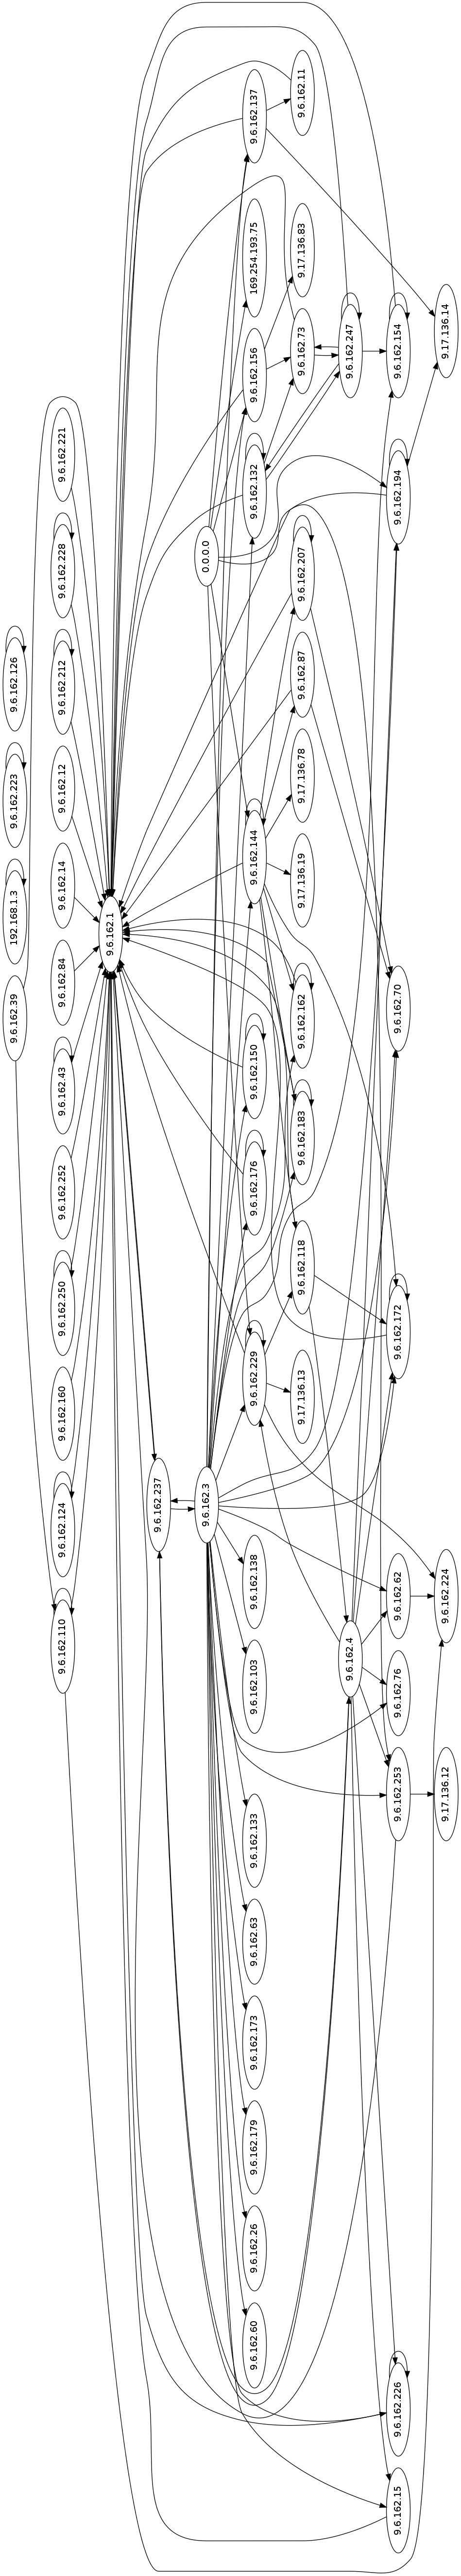
\includegraphics[height=0.90\textheight,keepaspectratio]{topologia.png}
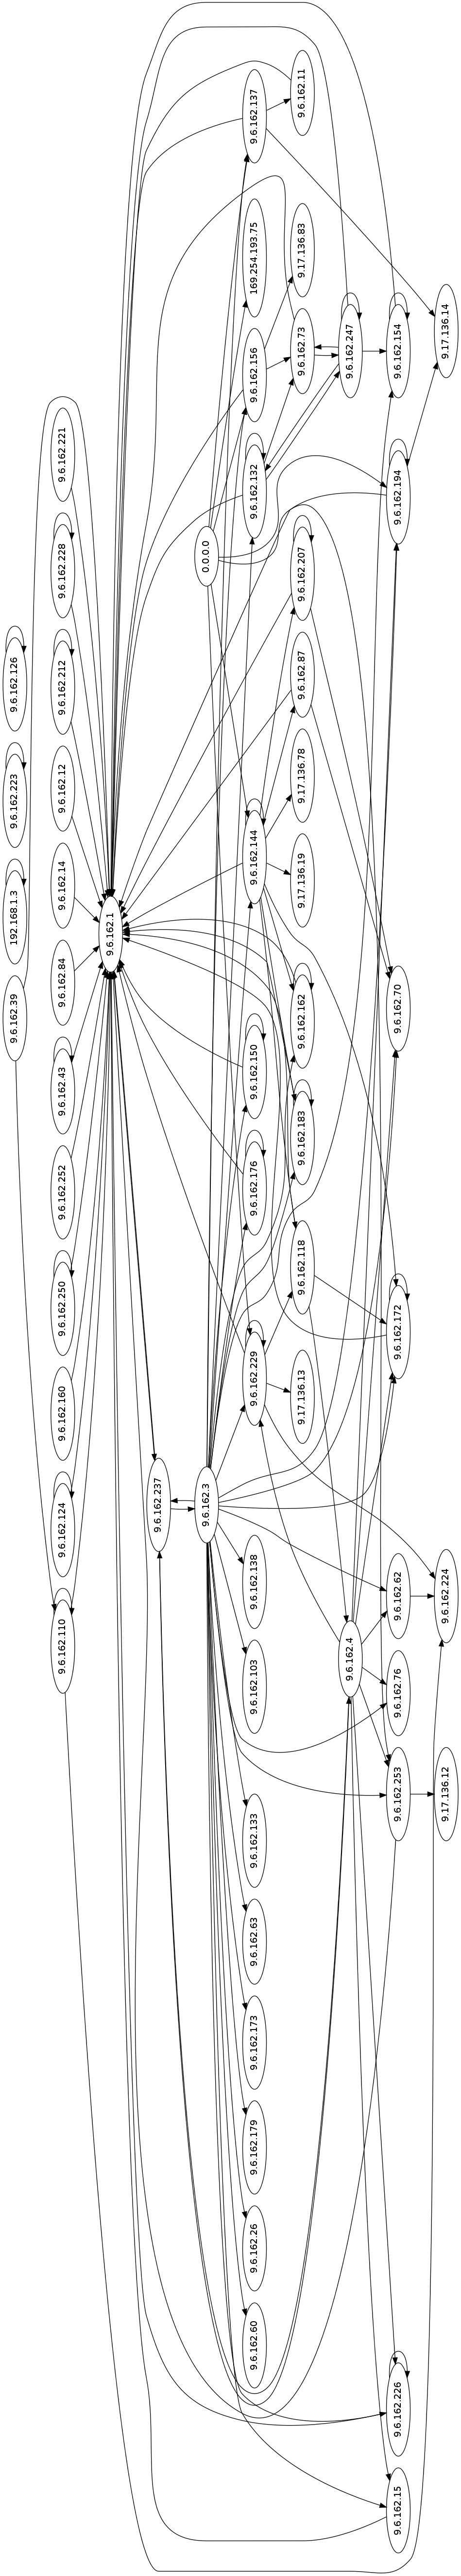
\includegraphics[height=0.90\textheight,width=0.90\textwidth]{topologia.eps}
\end{center}
\caption{Topolog'ia de la red analizada} \label{figura6}
\end{figure}

% volver a tener margenes normales
\restoregeometry

\end{document}

